%\section{Commonsense Knowledge Types}
\label{knowledge_types}
Intrigued by the achieved high accuracy of the Sharma and Baral \cite{2018CommonsenseKT} approach, we now describe this work in more detail. In section \ref{section:TheDifferentApproaches} we outlined \underline{\ref{Steps}} of this approach. Here, we first focus on the process of identification of the presented commonsense knowledge types. Then, we discuss the proposed reasoning algorithm and the provided worked out example. We conclude this chapter with some final observations about this approach.


\section{Identification of Commonsense Knowledge Types}
The first step of the Sharma and Baral \cite{2018CommonsenseKT} approach is to represent the input Winograd sentence and question as semantic graphs. To achieve this, the KParser from \cite{DBLP:conf/ijcai/SharmaVAB15} is used. 
To illustrate the results of the semantic parsing, we analyze part of a WS which is shown in \ref{ex:Graph}.  \\ 
\labeltext{\textit{Example~3.1.1}}{ex:Graph}:
\begin{itemize}
	\item[\textbf{S:}] \textbf{The man could not lift his son because he was weak.}
	\item[\textbf{Q:}] \textbf{Who was weak?}
\end{itemize}

The  resulting graphs are shown in Figure \ref{Graph11} and Figure \ref{Graph12}.
In these graphs, the different colors of the nodes indicate the predefined class of nodes to which they belong. 
Nodes with underlined text represent events which correspond to the verbs in the sentence. Nodes with bold text represent entities and qualities of entities, and the nodes with italic text represent conceptual classes. The labels on the directed edges are the semantic relations between the different nodes in the graph. The number next to a word refers to the position of the word in the sentence. 
\begin{figure} [h!]
	\centering
	%\documentclass[border=10pt]{standalone}
%\usepackage{tikz}
\tikzset{
	treenode/.style = {shape=rectangle, rounded corners,
		draw, align=center,
		top color=white, bottom color=blue!20},
	root/.style     = {treenode, font=\ttfamily\normalsize, bottom color=red!30},
	env/.style      = {treenode, font=\ttfamily\normalsize},
	dummy/.style    = {circle,draw},
	level 1/.style={sibling distance=6cm, level distance = 3em, label = 1pt },
	level 2/.style={sibling distance=2.3cm,level distance = 5em}, 
	level 3/.style={sibling distance=2cm},
	blueRed/.style={env, top color=blue, bottom color=red} 
}
%\begin{document}
	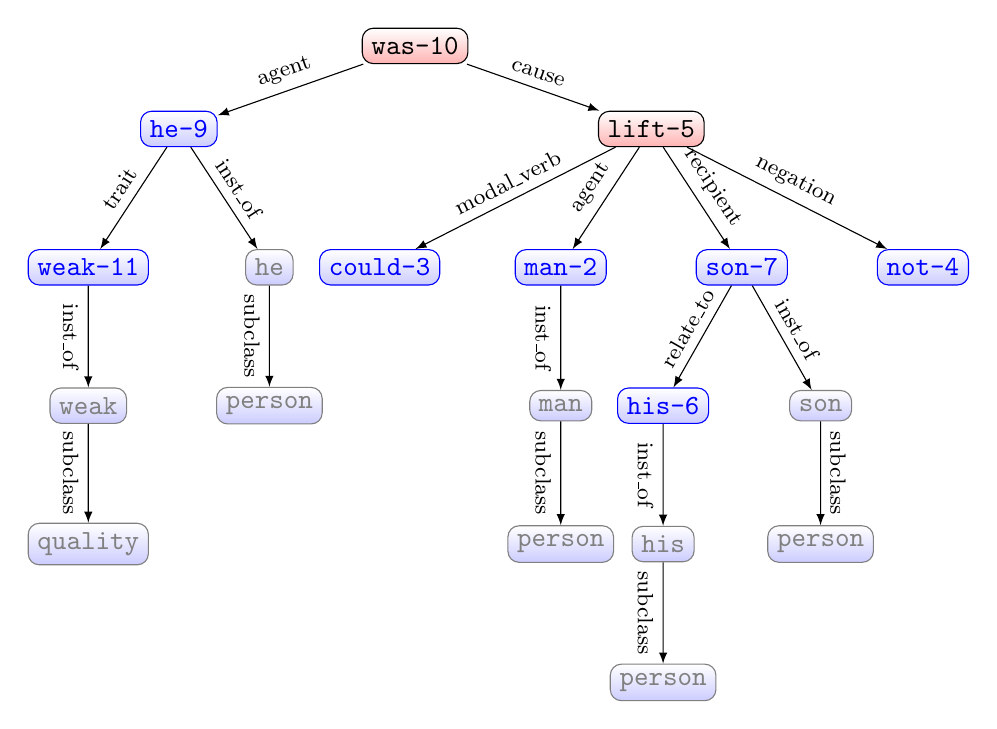
\begin{tikzpicture}
	[
	grow                    = down,
	sibling distance        = 50em,
	level distance          = 5em,
	edge from parent/.style = {draw, -latex},
	every node/.style       = {font=\footnotesize},
	sloped
	]
	\node [root] {was-10}
	child { node [env, blue] {he-9}
	  child {node [env, blue] {weak-11}
	  	 child {node [env, gray] {weak}
	  		child {node [env, gray] {quality}
	  			edge from parent node [below] {subclass}}
	  		edge from parent node [below] {inst\_of}}
			edge from parent node [above] {trait}}
	  child {node [env, gray] {he}
	  		child {node [env, gray] {person}
	  			edge from parent node [below] {subclass}}
	  		edge from parent node [above] {inst\_of}}	
	   edge from parent node [above] {agent}}
	child { node [env, bottom color=red!30] {lift-5} 
	  child {node [env, blue]  {could-3}
	  	edge from parent node [above] {modal\_verb} }	
	  child {node [env, blue]  {man-2}
	  	child {node [env, gray] {man}
	  		 child {node [env, gray] {person}
	  			edge from parent node [below] {subclass}}
	  		edge from parent node [below] {inst\_of}}
	  	edge from parent node [above] {agent} }
	  child {node [env, blue]  {son-7}
	  	child {node [env, blue] {his-6}
	  		child {node [env, gray] {his}
 			  	child {node [env, gray] {person}
  				   edge from parent node [below] {subclass}}
	  			edge from parent node [below] {inst\_of}}
	  		edge from parent node [above] {relate\_to}}
  		child {node [env, gray] {son}
  			child {node [env, gray] {person}
  				edge from parent node [above] {subclass}}
  		 edge from parent node [above] {inst\_of}}
	  	edge from parent node [above] {recipient}}
	  child {node [env, blue]  {not-4}
			edge from parent node [above] {negation} }
		edge from parent node [above] {cause}};
	

	\end{tikzpicture}
%\end{document}
	\caption{\label{Graph11}``The man couldn't lift his son because he was so weak."}
\end{figure}


\begin{figure} [h!]
	\centering
	%\documentclass[border=10pt]{standalone}
%\usepackage{tikz}
\tikzset{
	treenode/.style = {shape=rectangle, rounded corners,
		draw, align=center,
		top color=white, bottom color=blue!20},
	root/.style     = {treenode, font=\ttfamily\normalsize, bottom color=red!30},
	env/.style      = {treenode, font=\ttfamily\normalsize},
	dummy/.style    = {circle,draw},
	level 1/.style={sibling distance=3cm, level distance = 3em},
	level 2/.style={sibling distance=1.7cm,level distance = 5em}, 
	level 3/.style={sibling distance=2cm},
	blueRed/.style={env, top color=blue, bottom color=red} 
}
%\begin{document}
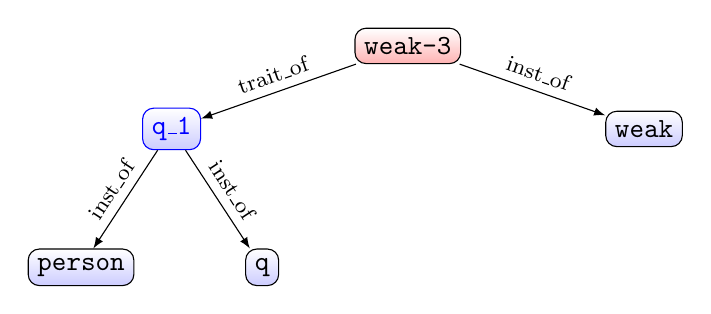
\begin{tikzpicture}
[
grow                    = down,
sibling distance        = 50em,
level distance          = 5em,
edge from parent/.style = {draw, -latex},
every node/.style       = {font=\footnotesize},
sloped
]
\node [root] {weak-3}
child { node [env, blue] {q\_1}
	child {node [env] {person}
		edge from parent node [above] {inst\_of}}
	child {node [env] {q}
		edge from parent node [above] {inst\_of}} 	
	edge from parent node [above] {trait\_of}}
child {node [env] {weak}
		edge from parent node[above] {inst\_of}};


\end{tikzpicture}
%\end{document}
	\caption{\label{Graph12}``Who was weak?"}
\end{figure}

\begin{figure} [h!]
	\centering
	%\documentclass{standalone}
%\usepackage{tikz}
%\usetikzlibrary{arrows, shapes, trees, positioning}

%\begin{document}
	
	\tikzset{
		treenode/.style = {shape=rectangle, rounded corners,
			draw, align=center,
			top color=white, bottom color=blue!20},
		root/.style     = {treenode, font=\ttfamily\normalsize},
		env/.style      = {treenode, font=\ttfamily\normalsize},
		dummy/.style    = {circle,draw},
		level 1/.style={sibling distance=6.3cm, level distance = 6em},
		level 2/.style={sibling distance=2.5cm,level distance = 5em}, 
		level 3/.style={sibling distance=2cm},
		blueRed/.style={env, top color=blue, bottom color=red} 
	}
	
	\begin{tikzpicture}
	[
	grow                    = down,
	sibling distance        = 50em,
	level distance          = 5em,
	edge from parent/.style = {draw, -latex},
	every node/.style       = {font=\footnotesize},
	sloped
	]
	
	
	
	% Theraspist 1
	\node[root]   (root)   {weak-1}
	child {node [env, gray] {weak}
		edge from parent node [above] {inst\_of}}
	child {node [env, gray] (s1) {y-2}
		child {node [env, gray] {entity}
			edge from parent node[above] {inst\_of}}
		edge from parent node[above] {is\_trait\_of}
	} ;
	
	
	
	% Theraspist 2
	\node[root]   (lift)   [right=45mm of root] {lifts-5}
	child {node [root] (s1) {y-2}
		edge from parent node[above] {agent}}
	child {node[env, gray] (S4) {lift}
		edge from parent node[above] {inst\_of}};
	
	\draw[-> ] (root) -- node[above] {prevents} (lift);
	%\draw[-> ] (lift) -- node[above] {agent} (s1);
	
	\end{tikzpicture}
%\end{document}
	\caption{\label{Graph13} ``weak y prevents y lifts"}
\end{figure}

\begin{figure} [h!]
	\centering
	%\documentclass{standalone}
%\usepackage{tikz}
%\usetikzlibrary{arrows, shapes, trees, positioning}

%\begin{document}
	
\tikzset{
	treenode/.style = {shape=rectangle, rounded corners,
		draw, align=center,
		top color=white, bottom color=blue!20},
	root/.style     = {treenode, font=\ttfamily\normalsize},
	env/.style      = {treenode, font=\ttfamily\normalsize},
	dummy/.style    = {circle,draw},
	level 1/.style={sibling distance=2cm, level distance =8em},
	level 2/.style={sibling distance=6cm,level distance = 5em}, 
	level 3/.style={sibling distance=2cm},
	blueRed/.style={env, top color=blue, bottom color=red} 
}
	
\begin{tikzpicture}
	[
	grow                    = down,
	%sibling distance        = 50em,
	level distance          = 5em,
	edge from parent/.style = {draw, -latex},
	every node/.style       = {font=\footnotesize},
	sloped
	]
		
	% Theraspist 1
\node [root] (root) {\underline{weak-12}}
child {node [env] {\textit{weak}}
		edge from parent node [above] {inst\_of}}
child {node [env]  {\textbf{so-11}}
	child {node [env] (so) {\textit{so}}		
		edge from parent node [above] {inst\_of} }
	edge from parent node [above] {modifier} }



;
	
	
	
	% Theraspist 2
	\node[root]   (lift)   [right=45mm of root] {\underline{lifts-5}}
	
	child {node [env] (son) {\textbf{son-7}}
		child {node [env] [right=35mm of so] {\textbf{his-6}}
			child {node [env] (person) {\textit{person}}
				edge from parent node [below] {inst\_of}}
		edge from parent node [above] {relate\_to}}	
		edge from parent node [above] {recipient}}
	child {node [env] (man) [right=10mm of so]{\textbf{man-2}}
		edge from parent node [above] {agent} }	
	child { node [env] (he) [right=7mm of son] {\textbf{he-9}}
		edge from parent node [above] {agent}}
	child {node[env] (S4) [right=20mm of son]  {\textit{lift}}
		edge from parent node[above, midway] {inst\_of}};
	
	\draw[-> ] (root) -- node[above] {prevents} (lift);
	\draw[-> ] (son) -- node[above] {inst\_of} (person);
	\draw[-> ] (man) -- node[above] {inst\_of} (person);
	\draw[-> ] (son) -- node[above] {inst\_of} (person);
	
	\draw[-> ] (root) -- node[above] {is\_trait\_of} (man);
	\draw[-> ] (root) -- node[above] {is\_trait\_of} (he);	
	
\end{tikzpicture}

%\end{document}
	\caption{\label{Graph14} Merged representation}
\end{figure}

For the representation of the question, one additional conceptual class labeled as "q" is introduced. In this conceptual class are the question words from the WSC problems, such as: \textit{Who, Which and What}. 
From the observation of these two graphs, Sharma and Baral \cite{2018CommonsenseKT} come to the conclusion that the missing knowledge required to answer the question, must connect the trait of an entity being weak with its inability to lift. Figure 3 depicts the representation of this knowledge as shown in \cite{2018CommonsenseKT}. 

By applying a similar analysis to all problems (285) from the WSC corpus \footnote{https://cs.nyu.edu/faculty/davise/papers/WinogradSchemas/WSCollection.xml}. Sharma and Baral \cite{2018CommonsenseKT} identified 12 different knowledge types. From these, the first 10 knowledge types share the same structure as they are all based on different interactions between actions and properties. Each of the 10 knowledge types consists of three parts: the first and third part are sentences containing entities, properties or actions, whereas the second part is a semantic relation (\textit{causes, prevents} or \textit{followed by}) which connects them. The last two knowledge types have a different structure because one of them requires multiple knowledge and the other one is based on the conditional likelihood of a previous event. 
For the representation of the knowledge type shown in Figure \ref{Ktypes} the first part is \textit{weak y}, the third part is \textit{y lifts} and the semantic relation is \textit{prevents}. The presented knowledge types are shown in Table \ref{Ktypes}. From the table, it can be noted that 240 problems (84\%) belong to the first 10 types and from these, 112(46\%) are in the 9th category. \\ 

\begin{figure} [h!]
	\centering
	

%\begin{tabular}{ |l|c|c|l| }
\begin{tabular}{ l | l }
    
    \textbf{Knowledge Type} & \textbf{\# of WSs} \\\hline
    1. Property \textit{prevents} Action  & 16 \\\hline
    2. Action1 \textit{prevents} Action2  & 6 \\\hline
    3. Action1 \textit{causes} Action2 & 41 \\\hline
    4. Property \textit{causes} Action & 27 \\\hline
    5. Action \textit{causes} Property & 13 \\\hline
    6. Property1 \textit{causes} Property2 & 4 \\\hline
    7. Action1 \textit{followed by} Action2  & 17\\\hline
    8. Action \textit{followed by} Property & 2 \\\hline
    9. Property \textit{followed by} Action &112 \\\hline
    10. Co-existing Action(s) and Property(s)& 2 \\\hline
    11. Statement1 \textit{is more likely than} Statement2 &26\\\hline
    12. Multiple Knowledge  &25 
\end{tabular}
%\end{tabular}



	\caption{\label{Ktypes} Knowledge types.}
\end{figure}
\pagebreak

\section{Reasoning Algorithm}
\label{RA}
In this section we explain the proposed logical Reasoning Algorithm (RA) from Sharma and Baral \cite{2018CommonsenseKT}. This RA was used for solving the WSC problems by applying the previously explained knowledge types. It takes a formal representation of the Winograd sentence, the question and the additional knowledge as input and it returns an answer to the question. The implementation of the RA together with a running example is available online\footnote{https://drive.google.com/file/d/1WN0T98HaMFhWEEIH-3AlWoIPxAdFYlT\_/view}. 

The RA is based on Answer Set Programming (ASP) \cite{DBLP:conf/aaai/Lifschitz08}. Therefore, after the Winograd sentence and question have been represented as semantic graphs, the observations from these graphs are encoded as ASP rules. The retrieved answer should be entailed by these input rules.
The RA is split into two main phases, each including several steps. The execution of each step results in new ASP rules. 
\begin{itemize}
	\item \textbf{Phase 1: Generating a merged representation}\\
	 In this phase, the graph representation of the Winograd sentence and the additional knowledge are merged. The idea here is to extend the information from the input sentence with the information from the additional knowledge. To achieve this, the following information from both graph representations is extracted and later merged.
	\begin{enumerate}
		\item All the nodes which are an instance of a defined class of nodes in the KParser (for example: person, motion, description), are identified as constant nodes. All constant nodes have a directed edge labeled as \textit{instance\_of} to another node in the graph. 
		\item Constant nodes with parents/children as constant nodes are identified. These are nodes previously identified as constant nodes which have directed edges to other constant nodes.
		\item The cross domain siblings in both representations are identified. These are different constant nodes which appear in both graphs and they both are instances of nodes of the same type. 
		\item Nodes which are identical in both graphs are identified. These nodes are called cross domain clones and are of the same type as the cross domain sibling. Additionally, they have the same number of child/parent nodes which are connected through the same semantic relations. 
		\item In this last step a merged representation is created. The merged representation is a copy of the sentence's representation, expanded with the additional knowledge by adding edges between nodes from both graphs that have been identified as cross domain clones.
	\end{enumerate}

	\item \textbf{Phase 2: Extracting possible answers}\\
	In this phase, the graph representation of the WSs question is projected onto the merged representation from the previous step. The goal is to retrieve the nodes which are cross domain clones of the unknown node (q) from the question in the merged representation. Similarly as in the previous phase, information from both graph representations is extracted and merged.
	\begin{enumerate}
		\item Constant nodes are identified from both graphs.
		\item Nodes with children/parent as constant node are identified. 
		\item Cross domain siblings of the nodes from the question graph are \\ identified in the merged representation.
		\item Using the previously extracted nodes, the cross domain clones of the nodes from\\ the question graph are identified in the merged representation.
		\item Nodes from the merged graph which are cross domain clones to the unknown node (q)\\ from the question graph are retrieved as an answer.
	\end{enumerate}
\end{itemize}
%TODO make the merged representation of the graph and refer to it in the text here
The implementation of the RA with the indicated phases and steps is available in Appendix \ref{AppendixA}. 
According to Sharma and Baral \cite{2018CommonsenseKT} this RA can be applied to WSC problems which belong to the first 10 from the identified 12 knowledge types. 

\paragraph{Worked-out example} To check the work of the RA, we run the code for the example which was provided together with the implementation of the RA in the supplementary document for Sharma and Baral \cite{2018CommonsenseKT}. This example illustrates the ASP encoding of the sentence and the question from \ref{ex:Graph}.
For extraction of additional knowledge the sentence \textit{``She could not lift it because she is a weak girl"} was used. The extracted knowledge from this sentence is \textit{``weak y prevent y lifts"} and this corresponds to the first knowledge type \textit{``Property prevents Action"}. The ASP encoding of this knowledge is shown in Code \ref{code}. The predicate name \textbf{has\_k} indicates that these rules are extracted from the graph representation of the additional knowledge. Similarly, there are predicates \textbf{has\_s} and \textbf{has\_q} for rules extracted from the graphs of the input sentence and question. Line 4 in Code \ref{code} is the rule which characterizes the corresponding knowledge type for this example. Running the RA with the provided ASP rules for the sentence, question and knowledge type, retrieves as answers: \textbf{ans(q\_1,he\_9)} and \textbf{ans(q\_1,man\_2)}. Hence, the two nodes \textbf{he\_9} and \textbf{man\_2} from the merged representation correspond to the unknown node \textbf{q\_1} from the question. The conclusion is that the correct referent for the ambiguous pronoun \textbf{he\_9} is the noun \textbf{man\_2}. 

\pagebreak
\begin{lstlisting}[language = Prolog, style=SC, caption={``weak y prevents y lifts"},label=code,numbers=left,
numberstyle=\tiny ]
has_k(weak_1,is_trait_of,y_2).
has_k(weak_1,instance_of,weak).
has_k(y_2,instance_of,entity).
has_k(weak_1,prevents,lifts_5).
has_k(lifts_5,instance_of,lift).
has_k(lifts_5,agent,y_2).
\end{lstlisting}


\paragraph{Observations}
After trying the provided worked out example and ensuring that the RA retrieved the correct answer, we decided to try out some more WSC problems (\#2, \#3, \#5, \#10, \#11, \#14, \#20, \#52 in Appendix \ref{AppendixB}).
In order to do this, we followed the same steps as for the worked out example. For each of the chosen WSC problems, as a first step we used the KParser to get the graph representation of the input Winograd sentence and question. Next, we encoded the relevant information from the graphs in ASP format. Since the knowledge types for the different WSC problems are not publicly available, we could not know the knowledge type of each of these problems. Therefore, we assumed that all the chosen problems correspond to the first knowledge type. For all of the chosen WSC problems we used the same rules as in Code \ref{code} as additional knowledge, where we only changed the traits and the events according to the Winograd sentences. For example, when considering the first half of the WS \#20, the trait is \textit{successful} and the event is \textit{envies}. To our surprise, for all of the WSs that we tried the correct answer was retrieved. This lead us to suspect that the rule for the identified knowledge type was not contributing at all to the reasoning procedure. 
To confirm this, on the worked out example we commented out the rule that defines the knowledge type (Line 4 in Code \ref{code}) and again the correct answer was retrieved. After trying both halves for all the chosen WSC problems, we came to conclusion that for extracting the answer, the RA relies on hard coded information about the agent and the recipient. For instance, if in Code \ref{code}, in Line 6 we substitute \textit{agent} with \textit{recipient}, the retrieved answer is then \textbf{ans(q\_1,he\_9)} and \textbf{ans(q\_1,son\_7)}.
Therefore, the conclusion of our observation is that the RA does not consider the rule for the knowledge type in the reasoning process. Rather, it relies on the hard coded information about the agent and the recipient of the main event for retrieving an answer. 

